\chapter{Calculus met Sympy}
\label{PC-Lab 1}
\graphicspath{{figures/Sympy/}}
The methods given in this course can be used to solve mathematical problems with pen and paper, but in practice this only works for relatively simple problems that require little computation, such as those covered in the board exercise sessions. Today, however, we usually leave the repetitive work to computers, which are specially designed to perform a huge number of calculations in a very short time.

Here we use the Python library Sympy. Sympy is a so-called computer algebra system capable of performing symbolic mathematical calculations on the computer. 
You can use Sympy to solve complex problems, but also to support and check your calculations when solving problems with pen and paper. First we give an introduction to using Jupyter, then we discuss in detail how Sympy can be used to (help) solve calculus problems.

\section{Jupyter Notebooks}
Jupyter uses so-called Notebooks, denoted by the .nipynb-extension, an interactive document containing both formatted text and code. This document is structured in what are known as \textbf{cells}. To create a new cell, you can press the plus sign on the top left.
Each cell has a particular style, which defines its properties and formatting. This style can be changed by pressing the drop-down menu at the top and selecting the desired style. We give a brief overview of the most commonly used cell styles.

\subsection{Code cell}
When we create a new cell in the Jupyter notebook, the default cell style is \textbf{Code}. In these cells we can enter mathematical operations, which can be performed with \keystroke{Ctrl}+\keystroke{Enter} (or by pressing \textbf{Run}). If the computation time gets too high (which often indicates a bug in the code), the evaluation can be aborted by pressing the square next to Run. The result of the evaluated Input cell is written out to a linked Output cell, which appears below it.

\begin{pyin}
1+1
\end{pyin}
\begin{pyout}
2
\end{pyout}

\subsection{Markdown}
\textbf{Markdown} cells contain formatted text and are used to provide explanations for the notebook.

\section{Sympy for dummies}
\label{sec:SympyTutorial}
This section goes over the basics of the Sympy language. Feel free to modify the following examples or experiment on your own!

\subsection{Operations, evaluations and lists}
\subsubsection{Mathematical and realtional operations}

\begin{tabular}{>{\hfill}p{5cm}p{12cm}}
	$+$ , $-$, $*$, $/$, $**$	&	Basic mathematical operators: sum, difference, multiplication, division, exponentiation\\
	$==,!=,>,>=,<,<=$	& relational operators: (un)equality, bigger than (or equal to), less than (or equal to)\\
	()				&	brackets to group operations\\
	\multicolumn{2}{l}{} 
\end{tabular}

Below we illustrate the use of some of these operators. 


\begin{pyin}
(10-5)*2**3
\end{pyin}
\begin{pyout}
40
\end{pyout}

\begin{pyin}
1 < 2 <= 3
\end{pyin}
\begin{pyout}
True
\end{pyout}

\begin{pyin}
5/2 == 10/3
\end{pyin}
\begin{pyout}
False
\end{pyout}


\subsubsection{Evaluation of expressions}

\begin{tabular}{>{\hfill}p{5cm}p{12cm}}
	\textit{expr} 			&	the exact result is shown in an Output cell below after executing the expression \textit{expr} \\
	\textit{N(expr)}	&	the numerical (approximate) result is given after executing the expression expr \\
	N(\textit{expr},\textit{n})			&	the numerical (approximate) result is given after executing the expression expr;
	With a precision of \textit{n} significant numbers in the Output cell\\
	\multicolumn{2}{l}{} 
\end{tabular}

\subsubsection{Assignements}
\begin{tabular}{>{\hfill}p{5cm}p{12cm}}
    \textit{x\_1, x\_2,\ldots = symbols('x\_1 x\_2 \ldots')}		&	this says that x\_1, x\_2, etc. are variables\\
	\textit{y = Function('y')(x)}		&	This says that y is a function of the variable x\\
	\textit{subs(x, value)}		&	This can be used to change the variable x with \textit{value}\\
	\multicolumn{2}{l}{} 
\end{tabular}

It should be noted that \textit{value} need not be a scalar value, but can equally be a symbolic expression.

We illustrate all this in the example below. 

\begin{example}
Save the expression $xy^2-2x(1+y^{-1})$ in the variable 	 \lstinline{expr}:
\begin{pyin}
x, y = symbols('x y')
expr = x*y**2-2*x*(1+1/y)
expr
\end{pyin}
\begin{pyout}
|$xy^2 - 2x\left(1+\frac{1}{y}\right)$|
\end{pyout}	
Evaluation of \lstinline{expr}, voor $x=y=1/3$, by direct assignment:
\begin{pyin}
expr.subs(x, 1/3).subs(y, 1/3)
\end{pyin}
\begin{pyout}
|$-2.62962962962963$|
\end{pyout}

Evaluation of \lstinline{expr}, for $x=3, y=2$ and $x= uv , y = u^2$, by exchange:
\begin{pyin}
expr.subs(x, 3).subs(y, 2)
\end{pyin}
\begin{pyout}
|$3$|
\end{pyout}
\begin{pyin}
u, v = symbols('u v')
expr.subs(x, u*v).subs(y, u**2)
\end{pyin}
\begin{pyout}
|$u^5v-2uv\left(1+\frac{1}{u^2}\right)$|
\end{pyout}
\end{example}

\subsubsection{Lists}
Often we want to work with several objects (values, functions ...) at the same time. This can be done by using lists:

\begin{tabular}{>{\hfill}p{6cm}p{11cm}}
	[e1, e2, ... ]		&	ordered sequence of elements e1, e2 \ldots\\
	\multicolumn{2}{l}{} 
\end{tabular}

Note that these elements can also be Lists themselves. Lists of lists are called \textbf{nested lists}. Lists can be used to pass multiple arguments to functions (see below), but can also be considered vectors. We can select elements from a list. For example, consider the vector v, then 

\begin{tabular}{>{\hfill}p{6cm}p{11cm}}
	\textit{v}[\textit{k}]		&		element \textit{k} in \textit{v} \\
	\multicolumn{2}{l}{} 
\end{tabular}


\begin{example}

Create the vector $\vec{v}_1=\begin{bmatrix}1\quad2\quad3\end{bmatrix}^T$ and select the first element.
	
\begin{pyin}
v1 = [1, 2, 3]
v1[0]
\end{pyin}
\begin{pyout}
1
\end{pyout}
\end{example}

\subsection{Functions}
\textbf{Functions} with arguments x, y, etc. are called as follows:

\begin{center}
	f(x,y,\ldots)
\end{center}
%\begin{tabular}{>{\hfill}p{5cm}p{12cm}}
%	f[x,y,\ldots]			&	 \\
%	\multicolumn{2}{l}{} 
%\end{tabular}

and entered:

\begin{center}
	f = lambda x\_,y\_,\ldots : \textit{expr}
\end{center}


where, \textit{expr} is an expression with the variables x, y \ldots .

\textbf{Implicit functions} can also be defined, but this requires specifying the dependent variables in \textit{expr} (see example).

\textbf{Piecewise functions} are implemented as follows:

\begin{center}
	f (\textit{x}\textunderscore ,\textit{ y}\textunderscore, ...) :=  Piecewise((\textit{expr1}, \textit{cond1}), (\textit{expr2}, \textit{cond2}), ...)
\end{center}


where \textit{expr1, expr2,}\ldots  are expressions with variables \textit{x, y,}\ldots and \textit{cond1, cond2,}\ldots the conditions they must satisfy. Indeterminate indicates that in the regions where the variables do not satisfy any of the conditions, f is undefined.
   
In addition to self-defined functions, Mathematica has numerous built-in functions:

\begin{tabular}{>{\hfill}m{9cm}p{8cm}}
	log(x)			&	$\ln(x)$\\
	log(x,b)		&	$\log_b(x)$\\
	exp(x)			&	$e^x$\\
	sin(x), cos(x), sec(x),  csc(x), tan(x), cot(x)							&	trigonometric functions\\
	asin(x),  acos(x), asec(x),  acsc(x)		&	inverse trigonometric functions \\
	atan(x), acot(x)			&	\\
	\ifanalysis
	sinh(x),  cosh(x), sech(x),  csch(x), tanh(x), coth(x)						&	hyperbolic functions \\
	asinh(x),  acosh(x), asech(x),  acsch(x)	&	inverse hyperbolic functions\\
	atanh(x), acoth(x)	&	\\\fi
	\multicolumn{2}{l}{}
\end{tabular}

Note that Sympy can work both symbolically and numerically. It always works with exact values, unless it is explicitly stated that it should work numerically. The latter can be done with \lstinline{//N} or \lstinline{N[expr]},  or by using a decimal.

Finally, we note that there are numerous other functions available in Sympy, such as the previously cited \lstinline|Piecewise|.


\begin{example}
Calculate $e^{\ln(x)}=x$:

\begin{pyin}
exp(log(x))
\end{pyin}
\begin{pyout}
|$x$|
\end{pyout}

Exact and numerical evaluation of $f(x) = \sin(x)^2/5$ for $x = 5$:
\begin{pyin}
	f = lambda x : sin(x)**2/5
	f(5)
\end{pyin}
\begin{pyout}
|$\frac{sin^2(5)}{5}$|
\end{pyout}
\begin{pyin}
	N(f(5))
\end{pyin}
\begin{pyout}
|$0.183907152907645$|
\end{pyout}
Once more the function: $f(x) = \sin(x)^2/5$, but numerically defined:

\begin{pyin}
	f = lambda x : N(sin(x)**2/5)
	f(5)
\end{pyin}
\begin{pyout}
|$0.183907152907645$|
\end{pyout}

	Implicitly defined function $\sin(y) + y^3 = 6-x^3:$
\begin{pyin}
    y = Function('y')(x)
    f = lambda a : sin(y.subs(x, a)) + y.subs(x, a)**3 - 6 + a**3
\end{pyin}
	Remark that $x$ is the only independent variable.
\begin{pyin}
    f(x)
\end{pyin}
\begin{pyout}
    |$x^3 + y^3(x) + sin(y(x)) - 6$|
\end{pyout}
\begin{pyin}
    f(2)
\end{pyin}
\begin{pyout}
    |$y^3(x) + sin(y(x)) + 2$|
\end{pyout}	
	A piecewise defined function:
\begin{pyin}
    f = Piecewise((x+1, x < 0), (-x**2+1, x > 0))
    f.subs(x, -0.5)
\end{pyin}
\begin{pyout}
    |$0.5$|
\end{pyout}
\begin{pyin}
    f.subs(x, 0)
\end{pyin}
\begin{pyout}
    |$NaN$|
\end{pyout}
\begin{pyin}
    f.subs(x, 0.5)
\end{pyin}
\begin{pyout}
    |$0.75$|
\end{pyout}
\end{example}

\subsection{Solving (un)equality's}
\begin{tabular}{>{\hfill}p{5cm}p{12cm}}
	solve(\textit{expr}, \textit{vars})		&	tries to find solutions of the equation, inequality, or system of equations/inequalities in \textit{expr} as a function of the variable \textit{vars}\\
	nsolve(\textit{expr}, \textit{vars})		&	tries to find a numerical approximation of the solutions of the equation, inequality, or system of equations/inequalities in \textit{expr} to the variables in \textit{vars}\\
	simplify(expr)			&	tries to find a simplified form of the expression in expr\\
	apart(expr)			&	splits the expression in expr into partial fractions\\
\end{tabular}

The results of \lstinline|solve| and \lstinline|nsolve| are given as lists.

\begin{example}
Find the exact and approximate values of the zero points of $x^2-2$:
\begin{pyin}
    expr = x**2-2
    extact = solve(expr, x)
    exact
\end{pyin}
\begin{pyout}
     |[-sqrt(2), sqrt(2)]|
\end{pyout}

\begin{pyin}
    numeric_1 = nsolve(expr, x, 1)
    numeric_1
\end{pyin}
\begin{pyout}
    |$1.4142135623731$|
\end{pyout}
\begin{pyin}
    numeric_2 = nsolve(expr, x, -1)
    numeric_2
\end{pyin}
\begin{pyout}
    |$-1.4142135623731$|
\end{pyout}
	Retrieve the first zero point from the list of solutions :
\begin{pyin}
    exact[0]
\end{pyin}
\begin{pyout}
    |$-\sqrt{2}$|
\end{pyout}
	The output of an unsolvable equation or system is an empty list.

\begin{pyin}
    solve([x**2-2, 2*x-5], x)
\end{pyin}
\begin{pyout}
    []
\end{pyout}
Split the fraction $\frac{x^2-2}{x+4}$ in partial fractions:

\begin{pyin}
    apart((x**2-2)/(x+4))
\end{pyin}
\begin{pyout}
    |$x-4+\frac{14}{x+4}$|
\end{pyout}
\end{example}

\subsubsection{Mathematical numbers}
We now show a couple of special mathematical numbers:
pi				:	$\pi$
oo			:	$\infty$
exp(1)			:	e
I				: 	$i$ (complex getal)


\subsection{Visualisation}
Finally, we go over some of the functions that serve to create plots.

\begin{tabular}{>{\hfill}p{8cm}p{9cm}}
	plot(\textit{f}(\textit{x}),($x,a,b$)) 					&	Create a plot of the function \textit{f} over the interval $[a,b]$\\
	
	plot(($f_1$(\textit{x}),$f_2$(\textit{x}),\ldots),($x,a,b$)) 	&	Creat a plot of the functions $f_1$ , $f_2$, \ldots over the interval $[a,b]$.\\
	
	plot3d($g(x, y),(x,a,b),(y,c,d)$]		&	Create a 3D plot of $g$ over the range \\&
	$[a,b]\times[c,d]$.\\
	%ListPlot[ \{\{$x_1,y_1$\},\{$x_2,y_2$\},\ldots\} ] 		&	Create a plot for the points $(x_i, y_i)$.\\
	
	plot\_implicit($g(x, y),(x,a,b),(y,c,d)$)	&	plot the contour(s) of $g$ over the range\\
	& $[a,b]\times[c,d]$ ($g$ can also be implicitly defined)\\
	plot\_implicit( $cond,(x,a,b),(y,c,d)$)	&	plot the subarea of $[a,b]\times[c,d]$ where the conditions in \textit{cond} are met\\
	
	plot\_parametric( $(k(u),l(u)),(u,u_{min},u_{max})$)	&	plot the parametric equations  $x = k(u)$ and $y =l(u)$ for $u\in[u_{min},u_{max}]$\\
	
	\multicolumn{2}{l}{} 
\end{tabular}

There are numerous options for customizing plot formatting.  Below we give an overview of the most important ones:

\begin{tabular}{>{\hfill}p{6.5cm}p{11cm}}
	title  -> "title" 					&	gives a title to the plot\\
	xlabel and ylabel -> "x" and "y"				&	labels the axes\\
	ylim -> \{\textit{ymin, ymax}\}			&	specifies the y-range of the plot\\
	size -> \textit{width, height})				&	specifies the width and height of the plot\\
	legend -> \{\textit{name1},  \textit{name2}, \ldots\}	&	creates a legend with the names of the plotted function\\
	\multicolumn{2}{l}{} 
\end{tabular}


\begin{example}
	Plot $\sin(x)$ the default layout: 
\begin{pyin}
    plot(sin(x), (x, 0, 2*pi))
\end{pyin}
\begin{pyout}
   |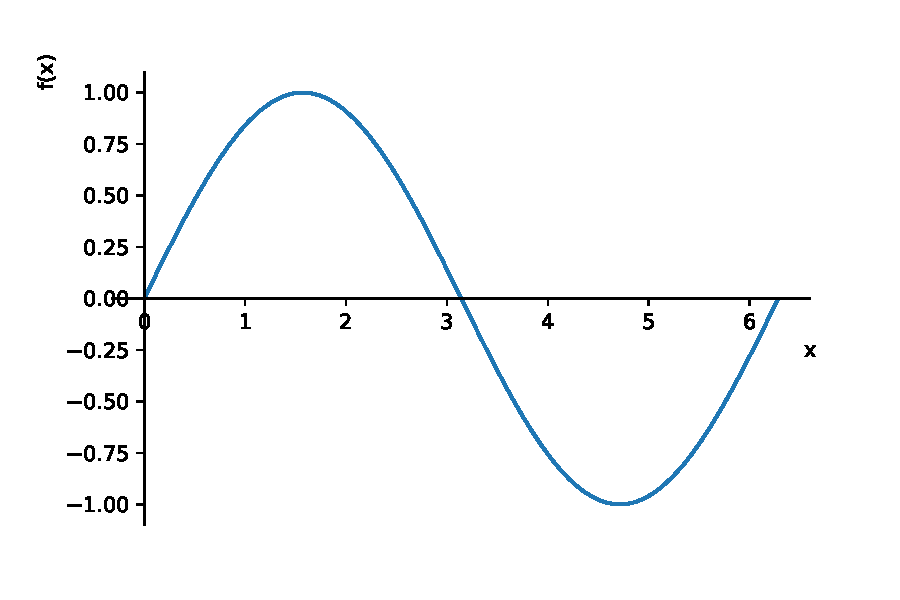
\includegraphics{figures/Sympy/fig_sympy_1.pdf}|
\end{pyout}
	Plot $\sin(x)$ with custom layout:
	
\begin{pyin}
    plot(sin(x), (x, 0, 2*pi), title='grafiek van sin(x)', xlabel='x', ylabel='y',
    ylim=(-1.5, 1.5), size=(10, 5))
\end{pyin}
\begin{pyout}
    |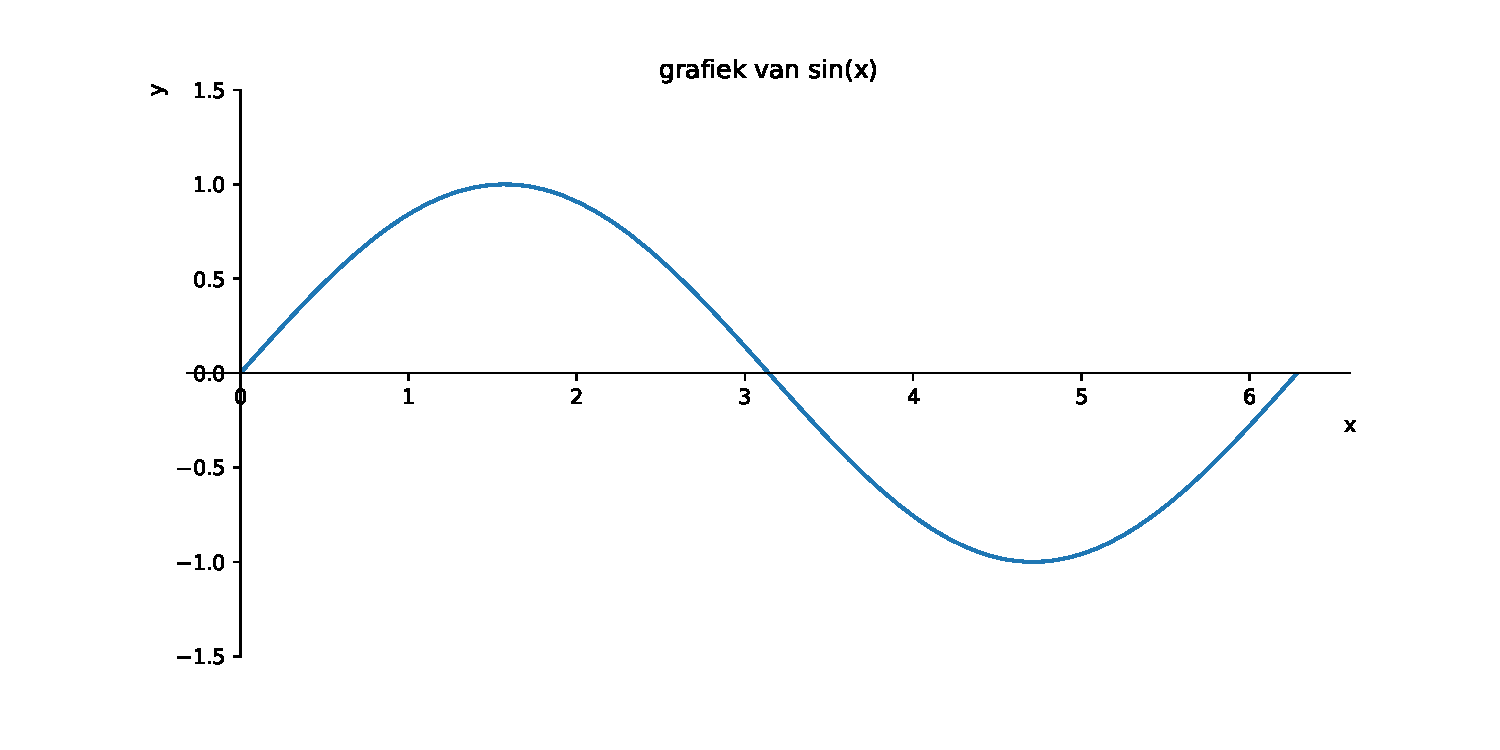
\includegraphics{figures/Sympy/fig_sympy_2.pdf}|
\end{pyout}

	Plot $\sin(x)$ en $cos(x)$ with custom layout:
	
\begin{pyin}
    graph = plot(sin(x), cos(x), (x, 0, 2*pi), title='grafiek van sin(x) en cos(x)',
    xlabel='x', ylabel='y', ylim=(-1.5, 1.5), size=(10, 5), legend=True, show=False)
    graph[0].line_color= 'b'
    graph[1].line_color='g'
    graph.show()
\end{pyin}
\begin{pyout}
    |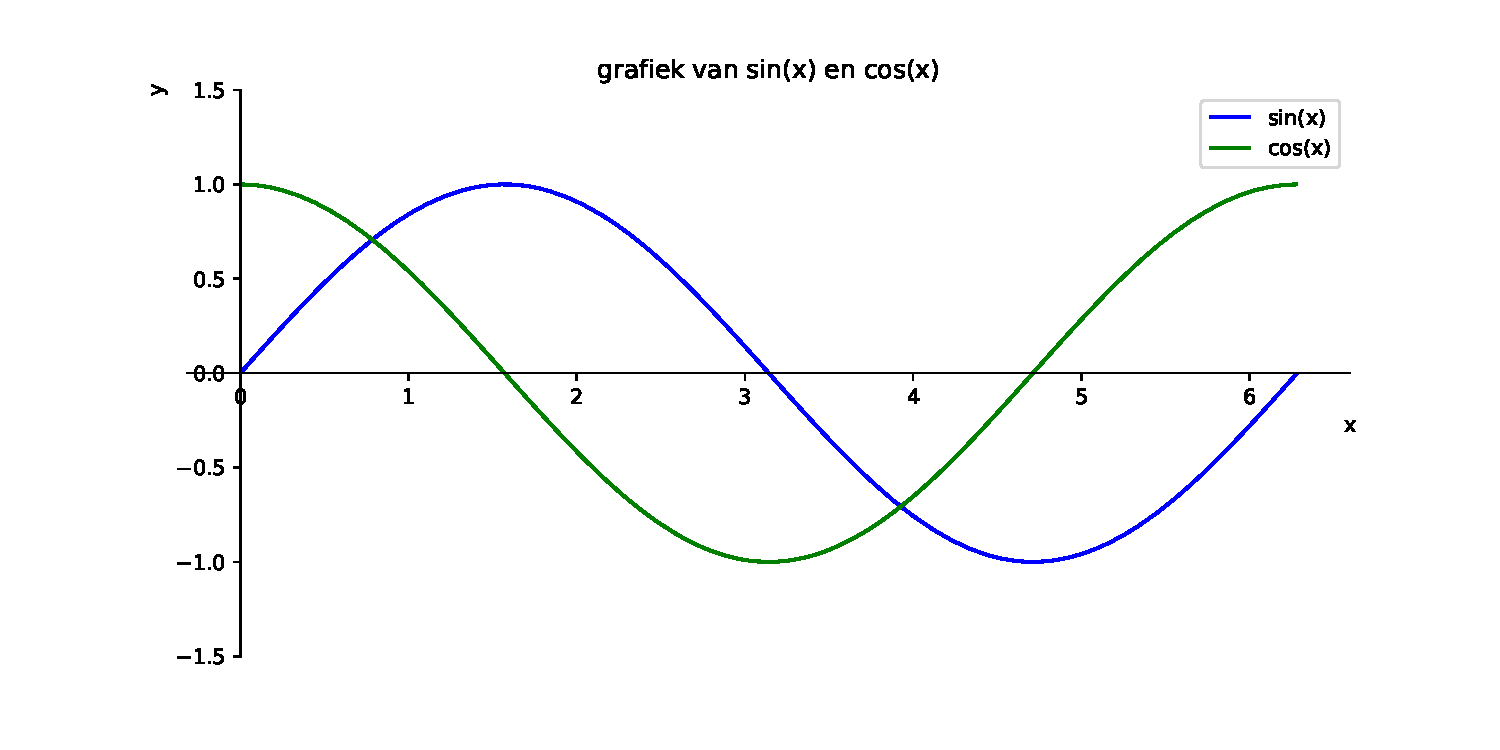
\includegraphics{figures/Sympy/fig_sympy_3.pdf}|
\end{pyout}

	Consider the function $g(x,y) = x^2+y^2$ over $[-5,5]\times[-5,5]$. Create a 3D and contour plot:
\begin{pyin}
    from sympy.plotting import plot3d
    x,y = symbols('x,y')
    plot3d(x**2+y**2, (x, -5, 5), (y, -5, 5))
\end{pyin}
\begin{pyout}
    |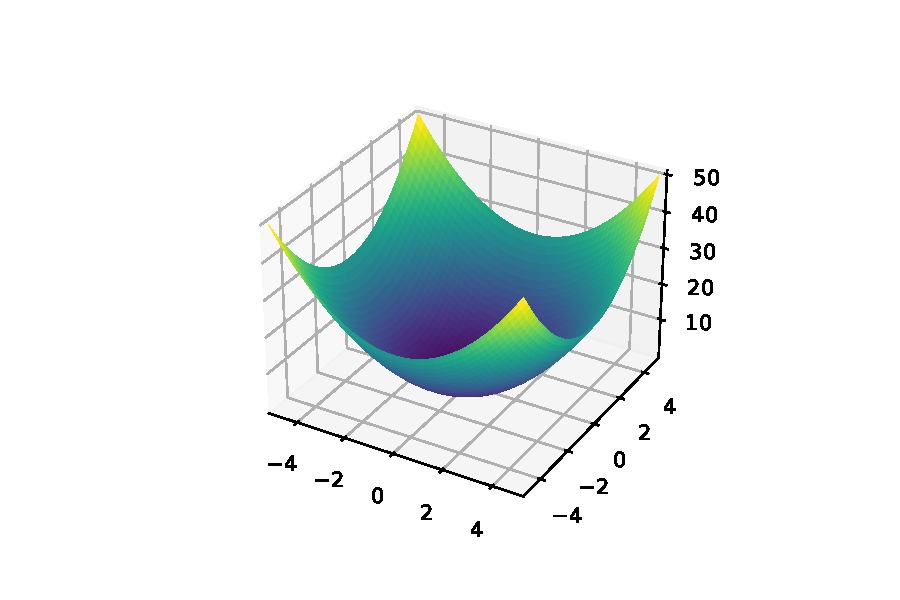
\includegraphics{figures/Sympy/fig_sympy_4.pdf}|
\end{pyout}

\begin{pyin}
    from sympy.plotting.plot import Plot, ContourSeries
    
    x,y = symbols('x,y')
    graph = Plot(ContourSeries((x**2 + y**2),(x,-5,5),(y,-5,5)))
    graph.show()
\end{pyin}
\begin{pyout}
    |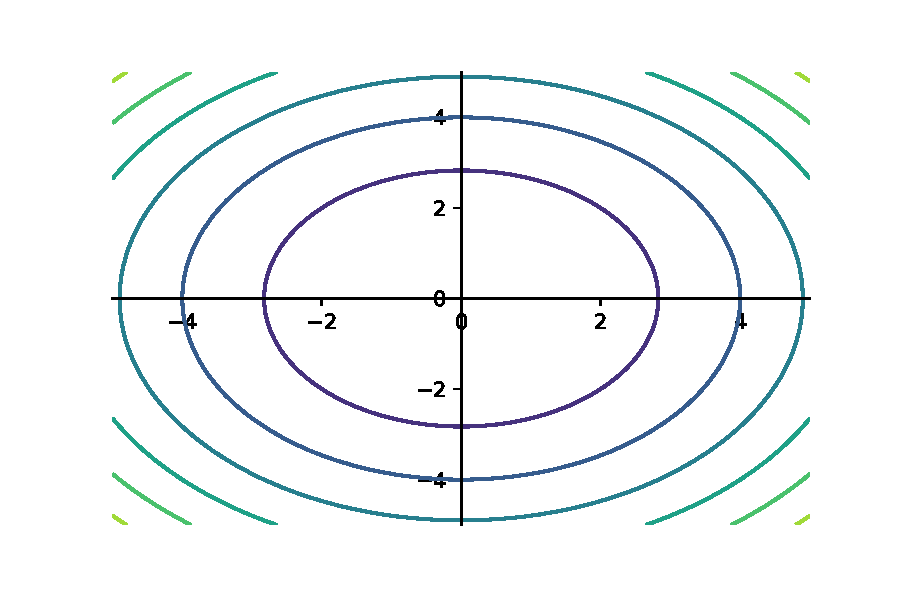
\includegraphics{figures/Sympy/fig_sympy_5.pdf}|
\end{pyout}
	Plot the circle of radius 2, using the implicit equation and the parametric equation:
	
\begin{pyin}
    plot_implicit(x**2+y**2-4, (x,-5,5),(y,-5,5))
\end{pyin}
\begin{pyout}
    |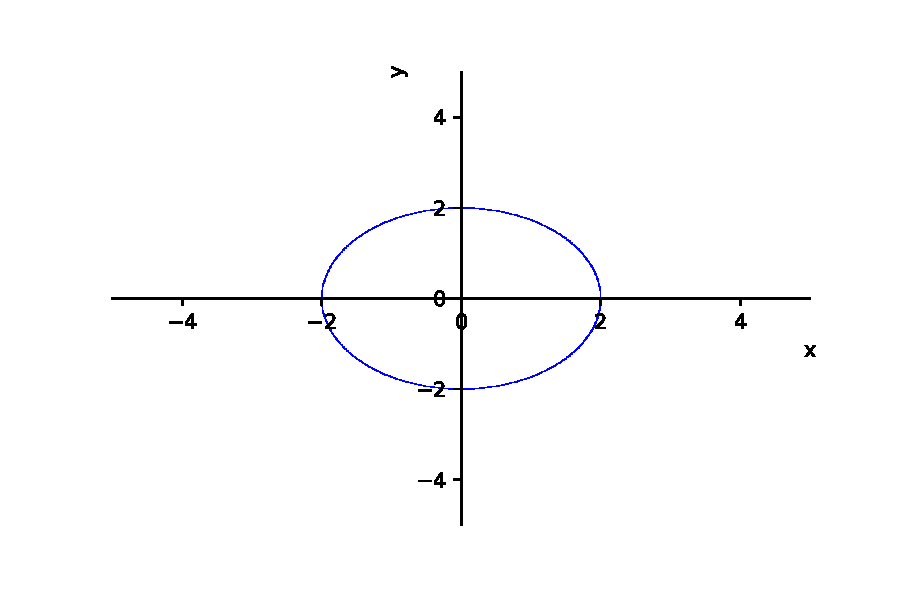
\includegraphics{figures/Sympy/fig_sympy_6.pdf}|
\end{pyout}

\begin{pyin}
    u = symbols('u')
    plot_parametric(2*cos(u), 2*sin(u),(u,0,2*pi))
\end{pyin}
\begin{pyout}
    |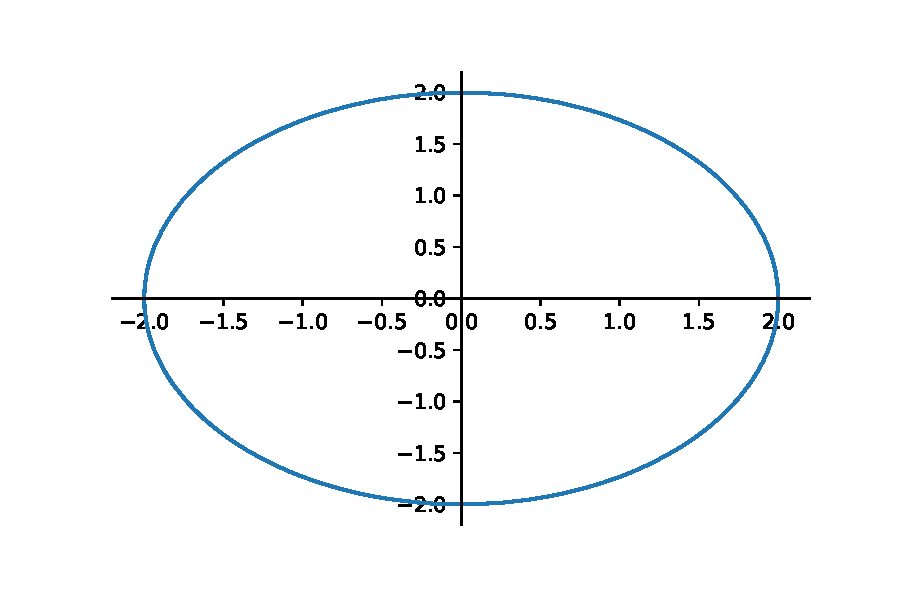
\includegraphics{figures/Sympy/fig_sympy_7.pdf}|
\end{pyout}

	Plot the subarea of  $[-5,5]\times[-5,5]$, delimited by the circle of radius 2:
	
\begin{pyin}
    plot_implicit(x**2+y**2 < 4, (x,-5,5),(y,-5,5))
\end{pyin}
\begin{pyout}
    |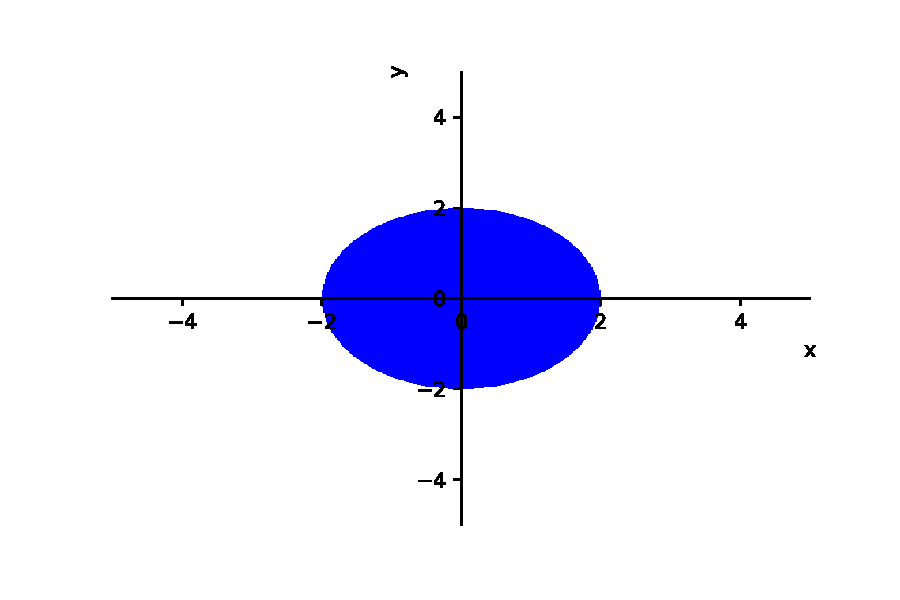
\includegraphics{figures/Sympy/fig_sympy_8.pdf}|
\end{pyout}
\end{example}


\section{Calculus specific intstructions}\label{sec:SympyAnalyse}

\subsection{Limits}
In Sympy we can calculate limits with the function \lstinline|Limit|.

\begin{tabular}{>{\hfill}p{8cm}p{9cm}}
	limit( $f(x)$, $x$, $c$)								&	determine the limit of $f$  in $c$\\
	limit($f (x)$, $x$, $c$, '+')		&	determine the right limit of $f$  in $c$ \\
	limit($f (x)$, $x$, $c$, '-')		&	determine the left limit of $f$  in $c$ \\
	\multicolumn{2}{l}{} 
\end{tabular}


\begin{example}
Determine the total, right and left limit of $1/x$ in $0$:
\begin{pyin}
    limit(1/x, x, 0)
\end{pyin}
\begin{pyout}
    |$\infty$|
\end{pyout}
\begin{pyin}
    limit(1/x, x, 0, '+')
\end{pyin}
\begin{pyout}
    |$\infty$|
\end{pyout}
\begin{pyin}
    limit(1/x, x, 0, '-')
\end{pyin}
\begin{pyout}
    |$-\infty$|
\end{pyout}

	Determine the limit of $1/x$ for $x \rightarrow +\infty$:
	
\begin{pyin}
    limit(1/x, x, oo)
\end{pyin}
\begin{pyout}
    |$0$|
\end{pyout}
\end{example}

\subsection{Derivatives}


Derivatives of functions with one variable can be calculated using \textbf{\lstinline|diff|}:\\

\begin{tabular}{>{\hfill}p{8cm}p{9cm}}
	diff($f(x), x$)			&			first order derivative of the function $f(x)$ towards $x$. For higher order derivatives you should enter x multiple times\\
	\multicolumn{2}{l}{} 
\end{tabular}


\begin{example}
Determine the first and second derivatives of $x^2+x$ :
	
\begin{pyin}
    f = lambda a : a**2+a
    diff(f(x), x)
\end{pyin}
\begin{pyout}
    |$2x+1$|
\end{pyout}
\begin{pyin}
    diff(f(x), x, x)
\end{pyin}
\begin{pyout}
    |$2$|
\end{pyout}

	We can keep the derivative as a function:

\begin{pyin}
    df = lambdify(x, diff(f(x), x))
    df(x)
\end{pyin}
\begin{pyout}
    |$2x+1$|
\end{pyout}

	Determine the derivative of the implicit function $y^3+y \sin =6-x^3$: 

\begin{pyin}
    x = symbols('x')
    y = Function('y')(x)
    fImpl = lambda a : sin(y)+y**3 - 6 + x**3
    diff(fImpl(x), x)
\end{pyin}
\begin{pyout}
    |$3x^2+3y^2(x)\frac{d}{dx}y(x)+cos(y(x))\frac{d}{dx}y(x)$|
\end{pyout}

	Try to rewrite the outcome in explicit form: 

\begin{pyin}
    solve(diff(fImpl(x), x), diff(y,x))
\end{pyin}
\begin{pyout}
    [-3*x**2/(3*y(x)**2 + cos(y(x)))]
\end{pyout}
\end{example}

With \lstinline{diff} we can also determine derivatives of functions of multiple variables:

\begin{tabular}{>{\hfill}p{8cm}p{9cm}}
	diff(f($x_1,x_2$,\ldots), $x_1$, $x_2$, \ldots			&			derivative of the function $f(x_1,x_2,\ldots)$. To derive multiple times to the same variable, you should enter that variable multiple times\\
	\multicolumn{2}{l}{} 
\end{tabular}

\begin{example}
Determine $f_x(x,y)$ and $f_{xy}(x,y)$ if $f(x,y) = x^2+xy+y^2$.
	
\begin{pyin}
    x, y = symbols('x y')
    f = lambda a, b : x**2+x*y+y**2
    diff(f(x, y), x)
\end{pyin}
\begin{pyout}
    |$2x+y$|
\end{pyout}
\begin{pyin}
    x, y = symbols('x y')
    f = lambda a, b : x**2+x*y+y**2
    diff(f(x, y), x, y)
\end{pyin}
\begin{pyout}
    |$1$|
\end{pyout}

Determine the gradient of $f(x,y) = x^2+xy+y^2$ in the point $(1,2)$.

\begin{pyin}
    f = lambda a, b : x**2+x*y+y**2
    grad = [diff(f(x,y),x), diff(f(x,y),x)]
    grad
\end{pyin}
\begin{pyout}
    |[2*x + y, 2*x + y]|
\end{pyout}

\begin{pyin}
    sol = []
    for g in grad:
        sol.append(g.subs(x, 1).subs(y, 2))
    sol
\end{pyin}
\begin{pyout}
    |[4, 5]|
\end{pyout}
\end{example}

\subsection{Integrals}
Sympy has one functions for integrating functions, being \lstinline{Integrate}.

\renewcommand{\arraystretch}{2.5}
\begin{tabular}{>{\hfill}p{5cm}p{12cm}}
	integrate$(f,x)$				&			determines the indefinite integral $\int f(x) dx$,\\
	integrate$(f,(x,a,b))$				&			determines the definite integral $ s\int^{b}_{a} f(x) dx$,\\
	\multicolumn{2}{l}{} 
\end{tabular}
\renewcommand{\arraystretch}{1}


\begin{example}
	Determine the following integral
	  $$ \ds\int\left(4x - x^2\right) dx.$$
\begin{pyin}
    integrate(4*x-x**2, x)
\end{pyin}
\begin{pyout}
    |$-\frac{x^3}{3}+2x^2$|
\end{pyout}
	Determine 
	 $$\ds\int\limits^{-\infty}_0 e^x dx.$$

\begin{pyin}
    integrate(exp(x), (x, 0, -oo))
\end{pyin}
\begin{pyout}
    |$-1$|
\end{pyout}

	Determine the numerical value of the definite integral  $$\ds\int\limits^{1}_0 \frac{\sin(x)}{x} dx.$$
	
\begin{pyin}
    N(integrate(sin(x)/x, (x, 0, 1)))
\end{pyin}
\begin{pyout}
    |$0.946083070367183$|
\end{pyout}
\end{example}

\subsection{Series}
We use following Sympy function to determine the Taylor series expansion of a function:	

\begin{tabular}{>{\hfill}p{5cm}p{12cm}}
	series($f,x,x_0,n$)						&			gives the taylor series expansion of $f(x)$ around $x_0$ with terms up to $n$-th order (+ the error term of the $n$-th order)\\
	\multicolumn{2}{l}{} 
\end{tabular}

\begin{example}
	Determine the Taylor series expansion of $\ln(x)$ in the area of  $x=1$ up to the $2-$the order term. 

\begin{pyin}
    s = series(log(x), x, 1, 3)
    s
\end{pyin}
\begin{pyout}
    |$-1-\frac{(x-1)^2}{2}+x+\mathcal{O}((x-1)^3; x\rightarrow1)$|
\end{pyout}

\begin{pyin}
    s.removeO()
\end{pyin}
\begin{pyout}
    |$x-\frac{(x-1)^2}{2}-1$|
\end{pyout}
\end{example}